\documentclass[runningheads]{llncs}
%
\usepackage{graphicx}
\usepackage{varioref}
\usepackage{float}
\usepackage{xurl}

\setcounter{secnumdepth}{4}
\setlength{\belowcaptionskip}{-16pt}

\begin{document}

\title{Speech emotion recognition}

\author{Francesco Tomaselli}
\authorrunning{F. Tomaselli}
\institute{University of Milan}
\maketitle

\begin{abstract}
    This study explores some techniques for audio classification, 
    comparing classical models and more advanced Neural networks. 
    A focus is putted on assessing the impact 
    of data augmentation.
    \keywords{Speech emotion recognition  \and Data augmentation}
\end{abstract}

\section{Introduction}

Speech emotion recognition is one of the many tasks that machine learning 
can tackle on audio signals. The requirement is, staring from raw audio files, 
to assign them an emotion, like neutral, happy or sad. 
As with many others classification tasks, one can follow a more classical 
approach, extracting features from raw files to capture important audio characteristics
and to build a classifier on top of that. 

Other methods are possibile, like using Convolutional neural networks on raw data, 
or deep learning networks with an high number of layers.

In contrast with other fields of work, audio with labelled emotions datasets are not
really big, this can be due to the fact that recording, preprocessing and validating 
emotions can be really expensive and time consuming, but it clearly creates an additional 
difficulty when trying to classify them. For this purpose, data augmentation takes a big role 
in this study as it can, if done right, mitigate the problems of data scarcity. 

\section{Methodology}

The proposed methodology can be summed in three main parts. 
The first step is audio preprocessing, we than add data augmentation, 
and lastly feature extraction.

The dataset picked for the study is the Ryerson Audio-Visual Database of Emotional Speech
and Song (RAVDESS). For the purpose of the project only speech audio files are 
considered.
Data is divided among 24 actors and 8 different emotions are present, namely: 
neutral, calm, happy, sad, angry, fearful, disgust and surprised.
Figure \ref{fig:classes} shows the classes distribution, we can see some imbalance. 
Data imbalance needs to be fixed during training, as a classifier could achieve an high accuracy 
score having terrible performance on underrepresented classes. 

There are many ways to tackle the problem, one is to augment the underrepresented classes, another 
one is to trim the dataset to have equal data distribution, and the last one is to use class weights 
during training. This last one is going to be the selected approach, it consists in multiplying 
the error on some classes by a factor, that takes into consideration the lower cardinality of 
some labels.  


\begin{figure}
  \begin{center}
      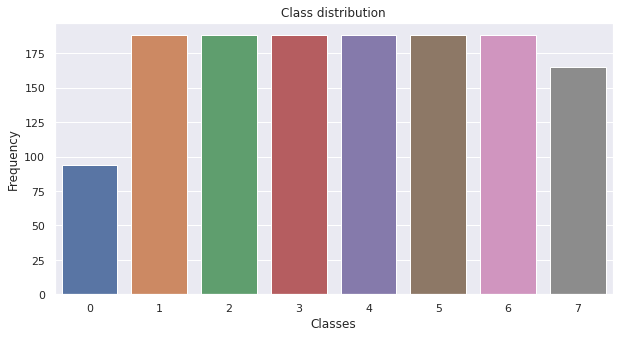
\includegraphics[width=0.7\textwidth]{images/classes.png}
      \caption{Dataset classes distribution.} \label{fig:classes}
  \end{center}
\end{figure}

\subsection{Feature extraction}

Before extracting features, we pad all audio files to the same length, 
that is the max of all the dataset. 
This is to avoid differences in dimensionality in later phases. The overall 
dataset duration distribution can be seen in Figure \ref{fig:dur}.

\begin{figure}
  \begin{center}
    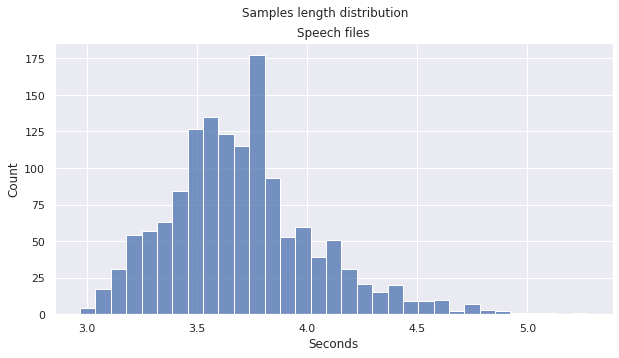
\includegraphics[width=0.7\textwidth]{images/duration.png}
    \caption{Audio duration distribution on the dataset.} \label{fig:dur}
  \end{center}
\end{figure}

\noindent After padding all the audio files to the same length, feature
extraction can take place.
The selected features are:
\begin{itemize}
  \item Pitches: pitches are extracted from the 
  files, we then can compute mean, std, max and min. Also, the pitch tuning offset is computed;
  \item Spectral centroid: after computing the spectral centroid, we normalize it
  and consider the mean, std and max;
  \item Flatness: another feature is the mean of the spectral flatness;
  \item MFCC: the first 50 mfcc are extracted and transposed. We then can consider
  the mean, std and max for each vector.
  \item Root-mean-square: the mean, max and std of the root-mean-square is computed.
\end{itemize} 
Finally, the mean of chromagram, melspectrogram, spectral contrast and zero crossing rate 
are considered.
A total of 312 features are obtained for each audio file. 

\noindent Figure \ref{fig:2d} shows a two-dimensional projection of the dataset, 
obtained using Principal component analysis on the extracted features, with the labels associated by K means.
K is set to $3$, found with the elbow method. The figure shows the difficulty of the task, indeed the 
we can see that clusters 0 and 1 have a great amount of labels associated with them, hence no 
real separation is present in the feature space.

\begin{figure}
  \begin{center}
    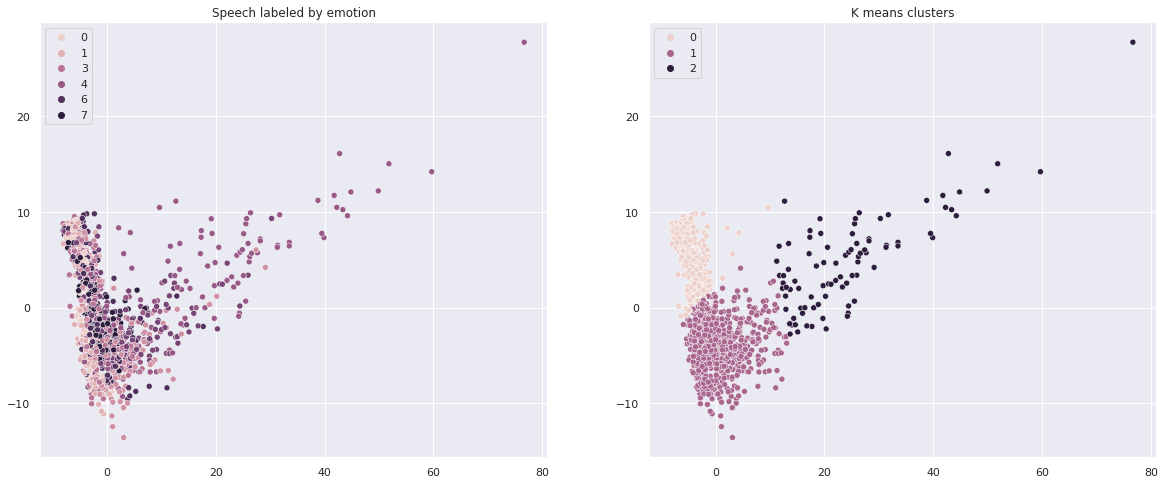
\includegraphics[width=\textwidth]{images/2d.png}
    \caption{Two-dimensional projection and K-means clusters of the extracted features.} \label{fig:2d}
  \end{center}
\end{figure}

\noindent After extracting features, they are scaled to have unit variance and 
zero mean. 
Also, Principal component analysis is an option, as it reduces dimensionality by 
keeping almost all the original variance of the data, the study on this 
part has been removed from the report as the performance is much worse with respect 
to keeping all the 312 features.

To train the Convolutional neural network, only the MFCC is uses, extracted in the same way 
discussed above.

\subsection{Data augmentation}

To avoid overfitting of the training set and potentially increase 
performances on the test set, a data augmentation phase is employed.
The goal is to increase the number of samples to help models with generalization. 
A raw audio is considered and a transformation is picked, the latter is parametrized to 
regulate the intensity of the change. 

\noindent The tree transformations used in the project are: 
\begin{itemize}
  \item Speed: audio is speed up or slowed down randomly. The ratio 
  in speed change goes from 0.6 to 1.4;
  \item Pitch: the pitch is shifted up or down randomly between -4 and +4 semitones;
  \item Noise: gaussian noise is added, the amplitude ranges from 0.0005 to 0.002.
\end{itemize}

\noindent Every augmenter is applied on the whole dataset, resulting 
is a cardinality that is four times the original.
Note that data augmentation happens only on the training split, the test one is 
always left untouched. 
An example of data augmentation can be seen in Figure \ref{fig:aug}. 

\begin{figure}[H]
  \begin{center}
    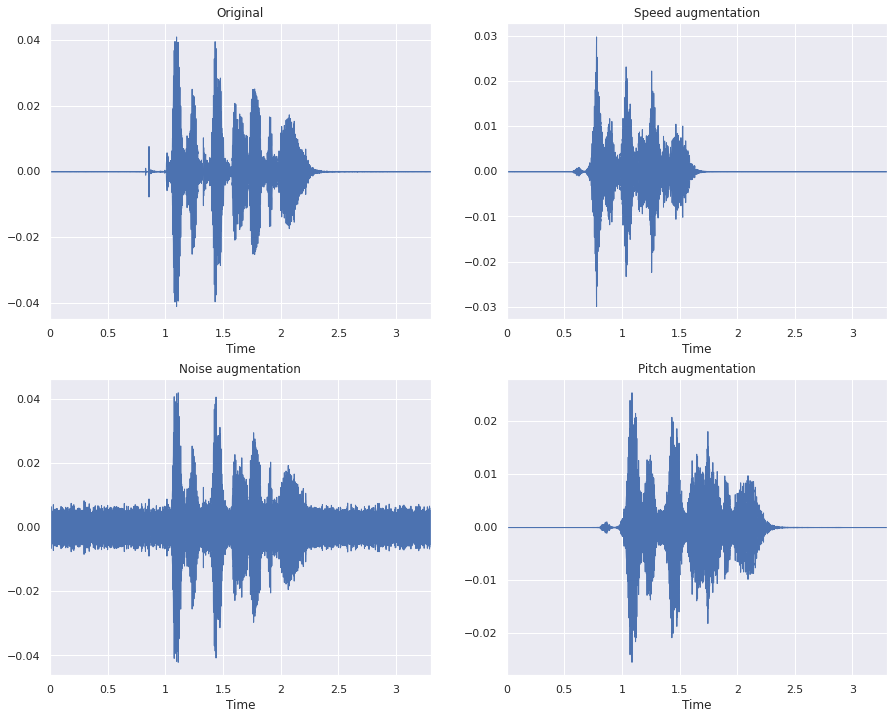
\includegraphics[width=0.9\textwidth]{images/aug.png}
    \caption{Data augmentation effects on example audio file.} \label{fig:aug}
  \end{center}
\end{figure}

\noindent One of the key factors when augmenting data is to keep the augmented samples plausible. 
Indeed, too much data augmentation result in training samples that do not help with generalization, 
while too little simply duplicates data in the training set.
The augmentation ranges are selected in an empirical way, after various tries. 

\section{Models definition}

The section talks about the models used in the study. 
We first start with classical ones and then focus on neural networks 
architectures.

\subsection{Classical models}
The classic models used are Support Vector Machines, K-NN and Decision trees.
The first one is left at default parameters, so the kernel is the radial basis function, 
regularization is set to one, gamma is set to scale. 
The choice of K for the nearest neighbors classifier is $\sqrt{|X|}$ where $X$ is the training set.
Lastly, the max number of levels of the decision tree is set to 10 to avoid 
over-fitting the data.

\subsection{Neural network}

A multilayer perceptron is used on the 312 features dataset. 
The architecture is quite simple at only four layers.
The first layer has 128 neurons, the second 64, the third 32 and lastly 8 
neurons for classification. 
All activation functions are relu, apart from the last that uses 
a softmax.
The Dense layers are separated by Dropouts with probability of 0.3.

The loss is the Sparse Categorical Cross-entropy, while the 
optimizer in use is the RMSprop with learning rate and decay
set to $5* 10^{-5}$ and $10^{-6}$ respectively.

\subsection{Convolutional Neural Network}

The Convolutional Neural Network that is trained of the MFCC is 
constructed as follows. 
Three blocks, each made of the following layers: 
\begin{itemize}
  \item 1D convolution: the number of filters is 32, 64 and 128, while the 
  kernel sizes are 8, 6 and 4 respectively.
  \item Batch normalization
  \item Relu activation
  \item Dropout
  \item 1D max pooling
\end{itemize}
The blocks are followed by a flatten layer, a 128 neurons Dense layer, 
Batch normalization and Relu activation. 
Finally, 8 neurons with sigmoid activation function outputs the predictions.
The optimizer and loss are the same as the ones used on the MLP.
\section{Experimental Results}

We now present the experimental results obtained on the dataset. 
The initial ones obtained with a random train test split, more specifically, 
70\% percent of the dataset is considered for the training, while the remaining part
for test. 
Out of that 70\%, a random 20\% is used for validation purposes.

\subsection{Training without augmentation}

After splitting the dataset randomly, SVM, K-NN and a Decision tree are trained and evaluated.
Those models do not perform really well compared to the neural networks in use.

The MLP and the CNN are trained with fit parameters on default, the number of epochs is quite high as
the learning rate for the optimizer is low to prevent a local minimum, they are 
1000 and 1500 respectively. The best model in terms of validation accuracy is saved 
and later loaded to obtain the accuracy results.

One factor in the training of the neural networks are the class weights. As can be seen 
in figure \ref{fig:classes}, there is a slight unbalance in the classes of the 
dataset. This would lead to poor performance on the under represented ones, thus 
class weights are computed and used during training.

The training results of the models can be seen in Table \ref{tab:res1}. 
MLP outperform other methods, while neural networks works better than simpler models.

\begin{table}
    \begin{center}
        \begin{tabular}{ |l|r| } 
        \hline
        Model & Accuracy \\
        \hline
        SVM   & 0.574 \\
        K-NN   & 0.400 \\
        Dtree & 0.381 \\
        MLP   & 0.645 \\
        CNN   & 0.633 \\
        \hline
        \end{tabular}
    \end{center}
    \caption{Training results without data augmentation.} \label{tab:res1}
\end{table}

\begin{figure}
    \begin{center}
      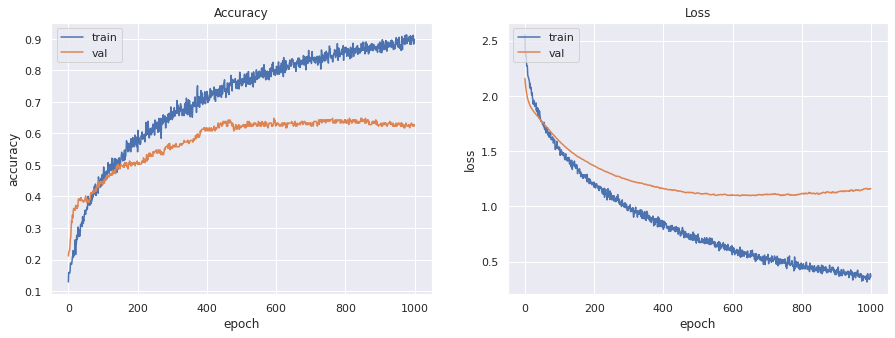
\includegraphics[width=\textwidth]{images/mlp1.png}
      \caption{Multilayer perceptron training progress on non-augmented data. Despite the 
      high number of epochs, dropout and a slow 
      learning rate prevents overfitting, as it only begin around epoch 600, 
      when the validation error start increasing.} \label{fig:mlp1}
    \end{center}
\end{figure}

\subsection{Training with data augmentation}

After testing the models without augmentation, speed, noise and pitch augmenters 
are used on the training set to enlarge it. 
As said before, the augmented data is used only on the training and validation set, 
while the randomly drawn test set remains in the original state.
The setup is exactly the same as before, so results can be compared. 
They can be seen in Table \ref{tab:res2}.

\begin{table}[H]
    \begin{center}
        \begin{tabular}{ |l|r|r| } 
        \hline
        Model & Accuracy w/o aug. & Accuracy w/ aug. \\
        \hline
        SVM   & 0.574  &  0.631 \\
        K-NN   & 0.400  &  0.414 \\
        Dtree & 0.381  &  0.428 \\
        MLP   & 0.645  &  0.659 \\
        CNN   & 0.633  &  0.668 \\
        \hline
        \end{tabular}
    \end{center}
    \caption{Training results with data augmentation.} \label{tab:res2}
\end{table}

\noindent Overall, every model performs better with data augmentation, the CNN is the best 
one, closely followed by MLP. An interesting note is that SVM with data augmentation 
has similar performances to CNN without data augmentation.

\subsection{Cross validation results}

The preliminary test on training with and without augmentation 
gives an idea about model performances, but to better evaluate them cross validation 
is required. 

The idea is to split the dataset in $K$ splits, train a model on $K-1$ splits
and evaluate on the latter. The process is repeated $K$ times and mean and standard deviation for
accuracy are computed. 
In this case, stratified cross validation with five folds is used. The stratified
version keeps in mind classes cardinalities when splitting the dataset, 
ensuring a similar distribution across all splits.
This method gives a better statistical estimation of the accuracy and loss, as 
splitting only once and obtaining a good results can be mostly luck-related.


To evaluate the impact of data augmentation, only the training splits are augmented, 
leaving the test split untouched, results can be seen in table \ref{tab:res3}.
The quantity in the parenthesis is the standard deviation.

\begin{table}[H]
    \begin{center}
        \begin{tabular}{ |l|r|r| } 
        \hline
        Model & Mean acc. w/o aug. (std) & Mean acc. w/ aug. (std)\\
        \hline
        SVM   &  0.588 (0.035)  &  0.643 (0.015) \\
        K-NN  &  0.441 (0.023)  &  0.422 (0.016) \\
        Dtree &  0.403 (0.036)  &  0.421 (0.041) \\
        MLP   &  0.611 (0.031)  &  0.692 (0.012) \\
        CNN   &  0.490 (0.058)  &  0.698 (0.030) \\
        \hline
        \end{tabular}
    \end{center}
    \caption{Cross validation results.} \label{tab:res3}
\end{table}

\noindent Again, data augmentation improves accuracy, but we can also see that the standard deviation is reduced
almost in all cases.
Also, the mean accuracy for CNN without data augmentation is drastically low 
with respect to the preliminary results obtained on the dataset, highlighting the importance
of performing cross validation.

\section{Concluding remarks}

This study explored audio speech emotion classification, comparing 
models trained on handcrafted features, and CNNs on MFCC.
A focus is putted on data augmentation and the results 
show how this procedure increases performance by a lot. 
Finally, cross validation is used to rank models between themselves.

Some possible future works involves exploring with additional 
augmentation, finding how much more data we can build from the dataset. 
Other models could be explored, like auto-encoders or LSTMs, as 
they perform really well on audio.

% \begin{thebibliography}{8}
% \bibitem{harvard_caselaw}
% Felix B. Chang, Erin McCabe and James Lee. ACL 2020. Mining the Harvard Caselaw Access Project.

% \bibitem{glda}
% Jagarlamudi Jagadeesh, Daum{\'e} III Hal and Udupa Raghavendra. ACL 2012. Incorporating Lexical Priors into Topic Models.

% \bibitem{hist-words}
% William L. Hamilton, Jure Leskovec, and Dan Jurafsky. ACL 2016. Diachronic Word Embeddings Reveal Statistical Laws of Semantic Change. 

% \bibitem{caselaw_query}
% Jaromir Savelka, Huihui Xu and Kevin D. Ashley. ACL 2019. Improving Sentence Retrieval from Case Law for Statutory Interpretation.

% \bibitem{argumentation_mining}
% Raquel Mochales and Marie-Francine Moens. ACL 2011. Argumentation Mining.

% \end{thebibliography}
\end{document}